% THIS IS AN EXAMPLE DOCUMENT FOR VLDB 2012
% based on ACM SIGPROC-SP.TEX VERSION 2.7
% Modified by  Gerald Weber <gerald@cs.auckland.ac.nz>
% Removed the requirement to include *bbl file in here. (AhmetSacan, Sep2012)
% Fixed the equation on page 3 to prevent line overflow. (AhmetSacan, Sep2012)
%
\def\sharedaffiliation{%
\end{tabular}
\begin{tabular}{c}}
%
\documentclass{vldb12}
%\usepackage{anysize}
%\usepackage{geometry}
%\geometry{top=1in, left=1in, right=1in, bottom=1in,footskip=.25in}
%\marginsize{1in}{0.8in}{1in}{1in}%tblr
%\usepackage[showframe,bottom=0.2in,footskip=.25in]{geometry}
%\usepackage[left=1in, right=1in, top=1in]{geometry}
%\newcommand{\cmt}[2]{\textcolor{dkmag}{[#1: #2]}}
%\newcommand{\personname}[1]{\cmt{Personname}{#1}}
%\newcommand{\standout}[1]{\textit{\textcolor{dkmag}{#1}}}
\usepackage{graphicx}
%\usepackage[draft]{hyperref}
\usepackage{epstopdf}
\usepackage{hyperref}
\usepackage{url}
%\usepackage{relsize}
\usepackage{caption}
\usepackage{alltt}
%\usepackage{multicol}
%\usepackage{lineno}
\usepackage{subcaption}
%\usepackage{subfloat}
%\usepackage{float}
\captionsetup[subfigure]{labelformat=brace}
%\usepackage{classicthesis}
%\usepackage[a4paper,bindingoffset=0.2in,left=1in,right=1in,top=1in,bottom=1in,footskip=.25in]{geometry}
%\usepackage[left=1in,right=1in,top=1in,bottom=0.5in,footskip=.25in]{geometry}
\usepackage{algpseudocode}
%\usepackage[bottom=0.8in]{geometry}
%\usepackage{lipsum}
\usepackage{amsmath,amssymb}
%\usepackage{color, MnSymbol} %, hyperref} %wrapfig,
%\usepackage{balance, multirow, framed, caption, subcaption}  % for  \balance command ON LAST PAGE
\usepackage{algorithm}
\usepackage{algpseudocode}
%\usepackage{array,multirow,graphicx,tabularx}
%\usepackage{aliascnt}
%\usepackage{relsize}
%\usepackage{titling}
%\usepackage{fullpage} %,enumitem}
%\usepackage[T1]{fontenc}
%\usepackage{enumitem}
%\usepackage[shortlabels]{enumitem}
%\setlist{nolistsep}
%\setlist[enumerate]{nosep}

%
%\usepackage{fancyhdr}
%\usepackage{fullpage} %, hyperref}
%\usepackage{amssymb, amsmath, enumitem, titling, hyperref}
%\usepackage[standard]{ntheorem}
%%\usepackage[sort&compress]{natbib}
%\usepackage[top=0.65in, bottom=1.2in, left=0.95in, right=0.95in]{geometry}
% %\ifthenelse{\value{page}=1}
%          %{\setlength\headheight{40pt}}
%          %{\setlength\headheight{0pt}}
%					
%\usepackage[backend=bibtex,sorting=anyt, maxnames=7, firstinits=true]{biblatex} %hyperref=true,
%\renewcommand*{\bibfont}{\footnotesize}
%\bibliography{bib_rs}
%%\renewcommand{\baselinestretch}{0.9}
\def\sharedaffiliation{%
\end{tabular}
\begin{tabular}{c}}

\newcommand{\bigCI}{\mathrel{\text{\scalebox{1.07}{$\perp\mkern-10mu\perp$}}}}
\newcommand{\nbigCI}{\cancel{\mathrel{\text{\scalebox{1.07}{$\perp\mkern-10mu\perp$}}}}}
\newcommand{\rred}[1]{\textcolor{red}{#1}}
\newcommand{\mc}[1]{\mathcal{#1}}
\newcommand{\ignore}[1]{}
\newcommand{\comlb}[1]{{\vspace{2mm}\noindent \rred{\bf COMM(Dan):}}~ #1 \hfill {\bf    END.}\\}
\newcommand{\combabak}[1]{{\vspace{4mm}\noindent \bf  COMM(Babak):}~ {\em \rred{#1}}\hfill {\bf END.}\\}


\newcommand{\reva}[1]{{{{#1}}}}
\newcommand{\revb}[1]{{{{#1}}}}
\newcommand{\revc}[1]{{{{#1}}}}



\newcommand{\dan}[1]{{{\color{magenta} Dan: [{#1}]}}}
\newcommand{\babak}[1]{{\texttt{\color{blue} Babak: [{#1}]}}}
\newcommand{\red}[1]{{\textbf {{\color{red} [{#1}]}}}}
\newcommand{\scream}[1]{{\texttt{\color{red}{\textbf{[{#1}]}}}}}


\newcommand{\att}{{\tau_{ATT}}}
\newcommand{\ate}{{\tau_{ATE}}}
\newcommand{\sch}{{\mathcal{S}}}
\newcommand{\rel}{{{R}}}
\newcommand{\sche}{{\mathcal{S}^e}}
\newcommand{\rele}{{{R}^e}}
\newcommand{\relei}{{{R}^e_{T_i}}}
\newcommand{\relt}{{{R}^e_{\trep}}}
\newcommand{\relti}{{{R}^e_{\trepi}}}
%\newcommand{\rel}{{{\textbf{R}}}}
\newcommand{\hm}{{\mathcal{S}}}
\newcommand{\crele}{{{R}^c}}
\newcommand{\echm}{{\mathcal{S}^{ce}}}
\newcommand{\cem}{{\textsc{Cem}}}
\newcommand{\mcem}{{\textsc{mCem}_{T_i}}}
\newcommand{\nnmwr}{{\textsc{Nnmwr}}}
\newcommand{\nnmnr}{{\textsc{Nnmnr}}}
\newcommand{\sbc}{{\textsc{SubC}}}
\newcommand{\prp}{{{P}_{\trep}}}
\newcommand{\prpi}{{{P}_{T_i}}}
\newcommand{\cv}{{{X}}}
\newcommand{\ccv}{{{\mc{X}}}}
\newcommand{\ccvi}{{{{cx}}}}
\newcommand{\cvi}{{{X_i}}}
\newcommand{\E}{\mathbb{E}}
\newcommand{\GSQL}{{{\textrm{ZaliQL}}}}
\newcommand{\delay}{\textsc{FlightDelay}}
\newcommand{\tre}{{{\mc{T}}}}
\newcommand{\trep}{S}
\newcommand{\trepi}{{{T}_i}}
\newcommand{\cvj}{{{X}_j}}
\newcommand{\cvij}{{{{X}}}}
\newcommand{\ccvj}{{\mc{X}}}
\newcommand{\ccvin}{{{\mc{X}'}}}
\newcommand{\ccvu}{{{\mc{X}}}}
\newcommand{\sub}{\bar{s}}
\newcommand{\LOGSPACE}{{\scriptsize $  \mathrm{LOGSPACE}$}}
\newcommand{\NLOGSPACE}{{\scriptsize $  \mathrm{NLOGSPACE}$}}
\newcommand{\PTIME}{{\scriptsize $  \mathrm{PTIME}$ }}

\newcommand{\ourproject}{{\textsc{Hume}}}
\newcommand{\ourlang}{{\textsc{HumeL}}}

\newcommand{\uiuc}{{UIUC}}
\newcommand{\cmu}{{CMU}}
\newcommand{\RP}{\emph{Robert Pennington}}
\newcommand{\TD}{\emph{Thomas Dunning}}

\newcommand{\ea}{\texttt{\bf E$_1$}}
\newcommand{\eb}{\texttt{\bf E$_2$}}
\newcommand{\ec}{\texttt{\bf E$_3$}}
\newcommand{\ed}{\texttt{\bf E$_4$}}
\newcommand{\ee}{\texttt{\bf E$_5$}}
\newcommand{\ef}{\texttt{\bf E$_6$}}

\newcommand{\Expl}{\texttt{Expl}}

\newcommand{\explq}{{explanation-query}}

\newcommand{\naivea}{\texttt{Alt-1}}
\newcommand{\naiveb}{\texttt{Alt-2}}
\newcommand{\incre}{\texttt{Incremental}}
\newcommand{\incrediff}{\texttt{Incremental-Diff}}

\newcommand{\tr}{1} %{\mathtt{t}}
\newcommand{\cn}{0} %{\mathtt{c}}




\newcommand{\A}{\texttt{A}}
\newcommand{\K}{\texttt{K}}
\newcommand{\deletelater}[1]{{\textbf {{\color{green} [{#1}]}}}}
\newcommand{\intervrel}{\texttt{intervened-relation}}
\newcommand{\attr}{\texttt{attr}}
\newcommand{\annot}{\texttt{annot}}
\newcommand{\supp}{\texttt{supp}}
\newcommand{\dom}{{\mathbb{D}}}
%\newcommand{\interv}{{\Gamma}}
\newcommand{\real}{{\mathbb{R}}}
\newcommand{\nat}{{\mathbb{N}}}
\newcommand{\explattr}{{\{E\}}}
%\newcommand{\change}{{\Delta}}
\newcommand{\bool}{{\textit{b}}}

\newcommand{\AP}{\texttt{AP}}
\newcommand{\highval}{\texttt{high}}
\newcommand{\midval}{\texttt{mid}}
\newcommand{\lowval}{\texttt{low}}
\newcommand{\aplow}{\texttt{poor}}
\newcommand{\aphigh}{\texttt{good}}
\newcommand{\dbnull}{\texttt{null}}
\newcommand{\relset}{\mathcal{R}}
\newcommand{\reltop}{{\mathcal{R}}_{top}}
\newcommand{\relbot}{{\mathcal{R}}_{bot}}
\newcommand{\attrset}{\mathcal{A}}
\newcommand{\attrtop}[1]{{\mathcal{A}}_{{top}, {#1}}}
\newcommand{\attrbot}{{\mathcal{A}}_{bot}}
%\newcommand{\featureset}{\mathcal{B}}
\newcommand{\db}{{D}}
\newcommand{\dbdom}{\mathbf{DB}}
\newcommand{\intervadditive}{{intervention-additive}}
\newcommand{\val}{{v}}
\newcommand{\valorig}{{u}}
%\newcommand{\dbdom}{\mathcal{D}}
\newcommand{\inputclass}{\mathcal{C}}
\newcommand{\intervene}{\mathcal{I}}
\newcommand{\tbaff}{{\tt{T_{Aff}}}}
\newcommand{\attaff}{{\tt{A_{Aff}}}}
\newcommand{\univ}{{{U}}}
\newcommand{\pk}{{\mathtt{pk}}}
\newcommand{\fk}{{\mathtt{fk}}}
\newcommand{\expl}{{\phi}}
%\newcommand{\pk}{{\tt \mathtt{\pk}}}
\newcommand{\sign}{{\tt \mathtt{sign}}}
%\newcommand{\expldom}{{\Phi}}
\newcommand{\select}{\tt {\textsc{Select}}}
\newcommand{\where}{{\tt \textsc{Where}}}
\newcommand{\with}{{\tt \textsc{With}}}
\newcommand{\distinct}{{\tt \textsc{distinct}}}
\newcommand{\groupby}{{\tt \textsc{Group By}}}
\newcommand{\from}{{\tt \textsc{From}}}
\newcommand{\ct}{{\tt \textsc{Count}}}
\newcommand{\create}{{\tt \textsc{Create}}}
\newcommand{\explanation}{{\tt \textsc{Explanation}}}
%\newcommand{\Pr}{{\tt {Pr}}}
\newcommand{\on}{{\tt \textsc{On}}}
\newcommand{\sqlwith}{{\tt \textsc{With}}}
\newcommand{\as}{{\tt \textsc{as}}}
\newcommand{\cascade}{{\tt \textsc{Cascade}}}
\newcommand{\sqland}{{\tt \textsc{And}}}
\newcommand{\sqlin}{{\tt \textsc{In}}}
\newcommand{\true}{{\tt true}}
\newcommand{\false}{{\tt false}}
\newcommand{\inmath}[1]{{\mathtt {#1}}}

\newcommand{\backwd}{\mathcal{B}}

\newcounter{enumQues}



\newcommand{\proj}[1]{{\Pi}}
\newcommand{\sel}[1]{{\sigma}}

\newcommand{\cut}[1]{}
\newcommand{\eat}[1]{}

%\newcommand{\tup}[1]{{\mathbf #1}}
\newcommand{\ul}[1]{{\underline{#1}}}
\newcommand{\commentresolved}[1]{}

\newenvironment{packed_item}{
\begin{itemize}
   \setlength{\itemsep}{1pt}
   \setlength{\parskip}{0pt}
   \setlength{\parsep}{0pt}
}
{\end{itemize}}

\newenvironment{packed_enum}{
\begin{enumerate}
   \setlength{\itemsep}{1pt}

  \setlength{\parskip}{0pt}
   \setlength{\parsep}{0pt}
}
{\end{enumerate}}

\newenvironment{packed_grep}{
\begin{description}
   \setlength{\itemsep}{1pt}
   \setlength{\parskip}{0pt}
   \setlength{\parsep}{0pt}
}
{\end{description}}

\newcommand{\ie}{{\em i.e.}} %\xspace}
\newcommand{\eg}{{\em e.g.}} %\xspace}
\newcommand{\etal}{{et al.}} %\xspace}
\newcommand{\aka}{{\em a.k.a.}\xspace}

\newcommand{\smalltt}{\tt \small}
\newcommand{\tinytt}{\tt \scriptsize}

\newcommand{\introparagraph}[1]{\textbf{#1.}}        % define own new subsection type: noindent, bold (textsc)

\newcommand{\angb}[1]{ {\langle {#1} \rangle}}                    % Set (as in \set{1,2,3}).

\newcommand{\set}[1]{\{#1\}}                    % Set (as in \set{1,2,3}).
\newcommand{\setof}[2]{\{{#1}\mid{#2}\}}        % Set (as in \setof{x}{x>0}).
\newcommand{\dtr}[0]{\twoheadrightarrow}        %
\newcommand{\bQ}[0]{\mathbf{Q}}        %
\newcommand{\bR}[0]{\mathbf{R}}        %
\newcommand{\bC}[0]{\mathbf{C}}
\newcommand{\bV}[0]{\mathbf{V}}
\newcommand{\mS}[0]{\mathcal{S}}
\newcommand{\mC}[0]{\mathcal{C}}
\newcommand{\bID}[0]{\mathbf{ID}}
\newcommand{\GCHQ}[0]{\textsc{GChQ}}
\newcommand{\CHQ}[0]{\textsc{ChQ}}
%\newtheorem{example}{Example}
%\newtheorem{pro}{Proposition}
%\newtheorem{proof}{Proof}
%\newtheorem{definition}{Definition}
%\newtheorem{theorem}{Theorem}
%\newtheorem{proposition}{Proposition}
%\newtheorem{def}{Definition}
%\usepackage[algoruled, lined]{algorithm2e}
%\usepackage{aliascnt}  		% ``hyperref’s \autoref command does not work well with theorems that share a counter:
						% it’ll always think it’s a Lemma even if it’s a Remark that shares the Lemma counter.
						% Load this package to fix it. No further intervention needed.''
						% Source: http://absatzen.de/thmtools.html (Jan 2009)
						% better: http://www.tug.org/applications/hyperref/manual.html (Nov 2009)
						% needs also: thm-patch.sty, parseargs.sty, aliasctr.sty ???
						% see section below for usage


\usepackage{graphicx}
\usepackage{balance}  % for  \balance command ON LAST PAGE  (only there!)

\begin{document}

% ****************** TITLE ****************************************

\title{ZaliQL: Causal Inference from Observational Data at Scale}
\numberofauthors{1}
\author{
  \alignauthor Babak Salimi  \ \  \ \ \  Corey Cole\ \  \ \ \    Dan R. K. Ports \ \  \ \ \  Dan Suciu
%
  \sharedaffiliation
  \affaddr{Department of Computer Science \& Engineering} \\
  \affaddr{University of Washington} \\
  \affaddr{\{bsalimi, drkp, suciu\}@cs.washington.edu, coreylc@uw.edu  }
}
% Ther
% possible, but not really needed or used for PVLDB:
%\subtitle{[Extended Abstract]
%\titlenote{A full version of this paper is available as\textit{Author's Guide to Preparing ACM SIG Proceedings Using \LaTeX$2_\epsilon$\ and BibTeX} at \texttt{www.acm.org/eaddress.htm}}}

% ****************** AUTHORS **************************************

% You need the command \numberofauthors to handle the 'placement
% and alignment' of the authors beneath the title.
%
% For aesthetic reasons, we recommend 'three authors at a time'
% i.e. three 'name/affiliation blocks' be placed beneath the title.
%
% NOTE: You are NOT restricted in how many 'rows' of
% "name/affiliations" may appear. We just ask that you restrict
% the number of 'columns' to three.
%
% Because of the available 'opening page real-estate'
% we ask you to refrain from putting more than six authors
% (two rows with three columns) beneath the article title.
% More than six makes the first-page appear very cluttered indeed.
%
% Use the \alignauthor commands to handle the names
% and affiliations for an 'aesthetic maximum' of six authors.
% Add names, affiliations, addresses for
% the seventh etc. author(s) as the argument for the
% \additionalauthors command.
% These 'additional authors' will be output/set for you
% without further effort on your part as the last section in
% the body of your article BEFORE References or any Appendices.

%\numberofauthors{4} %  in this sample file, there are a *total*
% of EIGHT authors. SIX appear on the 'first-page' (for formatting
% reasons) and the remaining two appear in the \additionalauthors section.


% Three authors sharing the same affiliation.

% You can go ahead and credit any number of authors here,
% e.g. one 'row of three' or two rows (consisting of one row of three
% and a second row of one, two or three).
%
% The command \alignauthor (no curly braces needed) should
% precede each author name, affiliation/snail-mail address and
% e-mail address. Additionally, tag each line of
% affiliation/address with \affaddr, and tag the
% e-mail address with \email.
%
% 1st. author

\frenchspacing


\maketitle

\begin{abstract}
Causal inference from observational data is a subject of active research and development in statistics and computer science. Many statistical software packages have been developed for this purpose.
However, these toolkits do not scale to large datasets.
We propose and demonstrate \GSQL: a SQL-based framework for drawing causal inference from observational data.
\GSQL\ supports the state-of-the-art methods for causal inference and runs at scale within PostgreSQL database system. \ignore{
\ignore{In addition, \GSQL\ includes several optimization techniques that significantly speedup causal inference, in both online and offline settings.}
\GSQL\ is designed as an extension for PostgreSQL database system.}
In addition, we built a visual interface to wrap around \GSQL. In our demonstration, we will use this GUI to show a live investigation of the causal effect of different weather conditions on flight delays.
\end{abstract}




\section{Introduction}
\label{sec:introduction}

% paragraph 1 before
\ignore{To this day, {\em randomized experiments} (A/B testing) remain the gold standard for causal inference.
However, in many domains, controlled experiments are not feasible for ethical, economical or practical reasons \cite{rosenbaum2002observational}.
Statistical methods for causal inference can be used to draw conclusions from {\em observational studies}, i.e., without controlled experiments  \cite{rosenbaum2002observational,Rubin2005\ignore{,PearlBook2000,Spirtes:book01}}. Computational, physical, and social scientists all increasingly want to perform causal inference on big data from observational studies:
%Big data is most commonly observational and highly relational (e.g,
social networks, biological networks, sensor networks and more.
Unfortunately, current software for processing observational data for causal inference does not scale. R, Stata, SAS, and SPSS have packages such as {\em MatchIt} and {\em CEM}~\cite{ho2005,iacus2009cem}, but they are designed for single-table data and are cumbersome with large datasets. For example, we found that running CEM on a dataset with 5M entries takes up to an hour using Stata, R or SAS.}

% paragraph 1 after
Randomized experiments (A/B testing) remain the gold standard for causal inference; however, they do pose a number of problems. Namely, controlled experiments are not feasible for ethical, economical, or practical reasons in a number of disciplines \cite{rosenbaum2002observational}. Observational studies can be used to draw causal inference without controlled experiments \cite{rosenbaum2002observational,Rubin2005,PearlBook2000\ignore{,Spirtes:book01}}.

%pararaph 2 after
Computational, physical, and social scientists all increasingly want to perform causal inference on big observational data, e.g., data from social networks and biological networks. Unfortunately, the current software for processing observational data in terms of causal inference cannot scale. R, Stata, SAS, and SPSS all have packages \cite{ho2005,iacus2009cem}; however, they are designed to be used only with single table data, making them cumbersome and often ineffective with large datasets. For example, we found performing CEM on a dataset with 5M entries takes up to an hour using Stata, R, or SAS. This is obviously not an effective practice for researchers.

%paragraph 2 before
\ignore{Additionally, causal analysis is part of a larger pipeline that includes data acquisition,  cleaning, and integration. For large datasets, these tasks are better handled by a relational database engine, which provides most of the functionality needed for these tasks, and also scales up to large datasets. %% \dans{the previous sentence is cumbersome.  what we want to say is that causal analysis is part of a larger pipeline that includes data acquisition, data cleaning, and data integration; for large datasets, these tasks are best handled by a relational database engine, which provides most of the functionality needed for these tasks, and also scales up to large datasets.}
}
% paragraph 3 after
Additionally, causal analysis is part of a larger pipeline that includes data acquisition, cleaning, and integration. For large datasets, these tasks are better handled by a relational database engine which provides most of the functionality needed for these tasks while also scaling up to large datasets.

%paragraph 3 before
\ignore {
In this demonstration, we propose \GSQL,\footnote{ The prefix Zali refers to
  al-Ghzali (1058-1111), a medieval Persian philosopher. It is known
  that David Hume (1711-1776), a Scottish philosopher, who gave the
  first explicit definition of causation in terms of counterfactuals,
  was heavily influenced by al-Ghzali's conception of causality.}
  a SQL-based framework for drawing causal inference within the DBMS. \GSQL\ takes the first step towards truly scalable causal inference by modeling it as a data management problem. We demonstrate that
  causal inference can be approached from this perspective, and that doing so is key to scalability and robustness.  \GSQL\ supports state-of-the-art methods for causal inference and runs at scale within a database engine.
}
% paragrpah 4 after
In this demonstration, we propose \GSQL,\footnote{ The prefix Zali refers to
  al-Ghzali (1058-1111), a medieval Persian philosopher. It is known
  that David Hume (1711-1776), a Scottish philosopher, who gave the
  first explicit definition of causation in terms of counterfactuals,
  was heavily influenced by al-Ghzali's conception of causality.}
  a SQL-based framework for drawing causal inference.  \GSQL\ takes the initial step towards scalable causal inference by modeling it as a data management problem. We show that causal inference can be approached from this perspective and that doing so is key for  scalable and robust causal analysis. \GSQL\ supports state-of-the-art methods for causal inference and runs at scale within a database engine.



\begin{figure}\center
 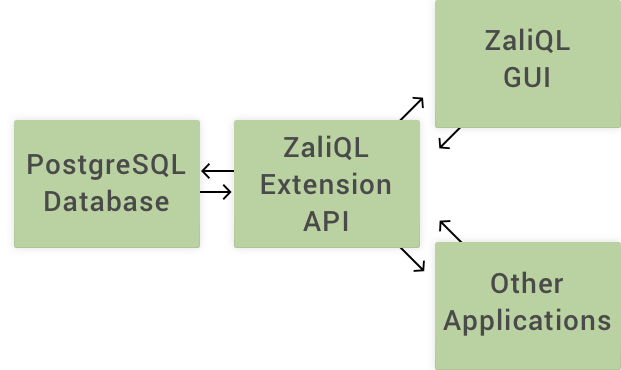
\includegraphics[scale=0.20]{Figures/System-Overview.png}
  \vspace{-3mm} \caption{ZaliQL architecture}

  \label{fig:arch}
  \vspace{-3mm}
\end{figure}

  \vspace*{-3mm}
\begin{figure} \center
  
\includegraphics[scale=0.21]{Figures/Matching-Flowchart.png}
  \vspace*{-4mm}\caption{Causal analysis workflow}

\label{fig:flowchart}
\vspace{-0.3cm}
\end{figure}

%\vspace{-.1cm}

\section{System Architecture}

% paragraph 1 before
\ignore{The overall architecture of \GSQL\ is shown in Fig. \ref{fig:arch}.
The API is a set of functions that support causal inference on data stored in a PostgreSQL DBMS.
The API will be packaged as a PostgreSQL extension.
The \GSQL\ API is modeled after the MatchIt and CEM toolkits
\cite{ho2005,iacus2009cem} and includes methods for drawing causal inference from relational data. For demonstration and exploration purposes, \GSQL\ also includes a web GUI
(see Fig. \ref{sfig:demo-tutorial}).
}
% paragraph 1 after
The overall architecture of ZaliQL can be seen in Fig. \ref{fig:arch}. The API is a set of functions that support causal inference on data stored in a PostgreSQL DBMS. The API will be packaged as a PostgreSQL extension. The ZaliQL API is modeled after the MatchIt and CEM toolkits \cite{ho2005,iacus2009cem} and includes methods for drawing causal inference from relational data. A web GUI is also included for demonstration and exploration purposes and is illustrated in Fig. \ref{sfig:demo-tutorial}.

\begin{figure*} \centering
\hspace*{-.1cm}
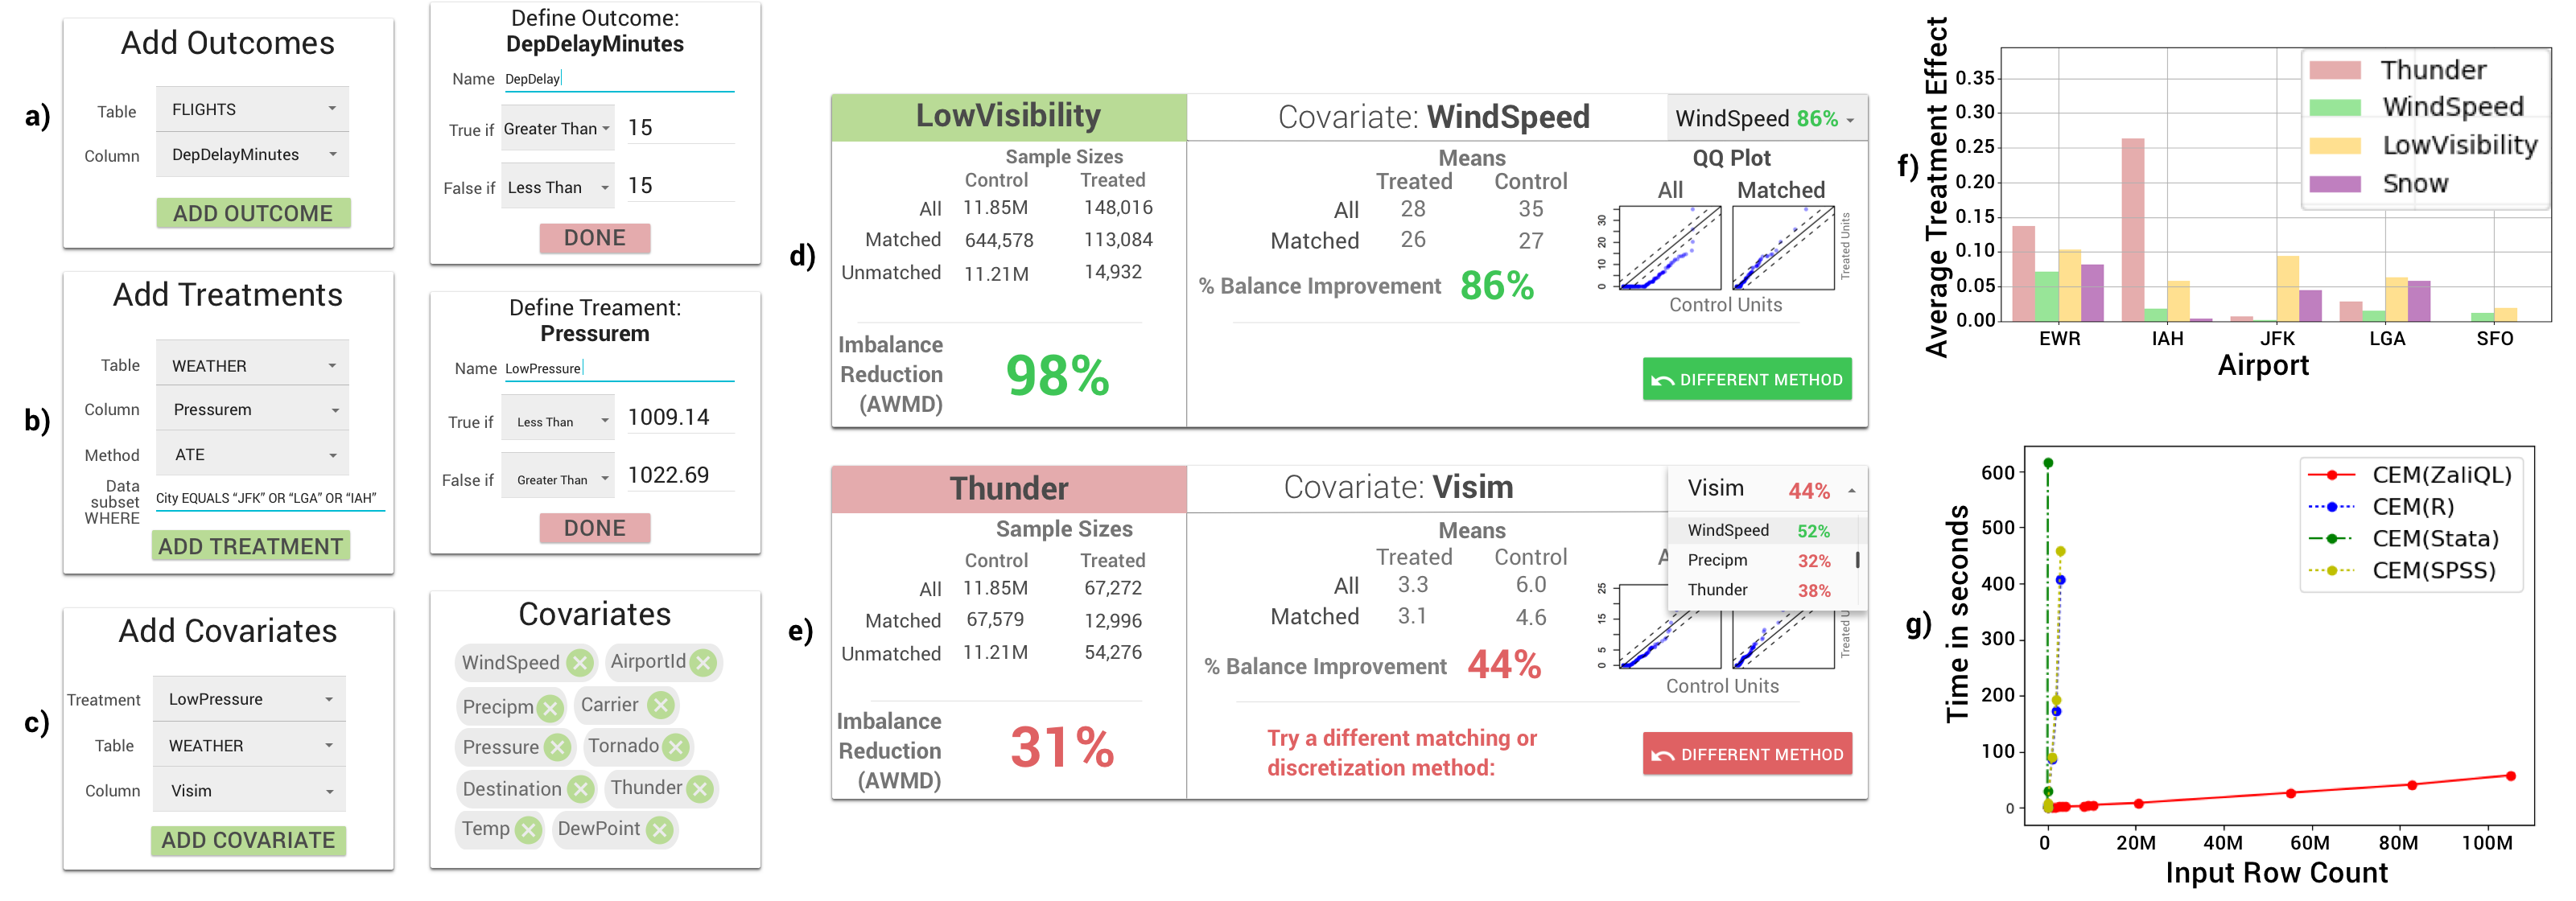
\includegraphics[scale=0.16]{Figures/Demo-Tutorial.png}
\caption{Demonstration screenshot described in Section \ref{sec:dd}}
\label{sfig:demo-tutorial}
\end{figure*}

\vspace{-.3cm}
\section{Demonstration Details}
\label{sec:dd}

% paragraph 1 before
\ignore {Modern causal analysis is an iterative process, as  illustrated in Fig \ref{fig:flowchart}.
An analyst acquires and integrates data from multiple sources,
generates a hypothesis, pre-processes the data with a matching  method (explained below), and then finally
 conducts the causal analysis. Frequently, this process needs to be repeated with a new matching
  method, a new hypothesis or new datasets \cite{IacKinPor09}.
  We demonstrate this workflow in \GSQL\ through several causal investigations on integrated flight and weather datasets.}
% paragraph 1 after
As the illustration in Fig. 2 shows, modern causal analysis is an iterative process. An analyst must acquire and integrate data from a myriad of sources, generate a hypothesis, pre-process the data through a matching method, and finally conduct the causal analysis. This linear process often must be repeated with new matching methods, new hypotheses, or even new datasets \cite{IacKinPor09}. Note that our system does not address the statistical validity of performing multiple hypothesis testing. We will demonstrate ZaliQL by providing walkthroughs using causal investigations on integrated flight and weather datasets.

% data before
\ignore{{\bf Data:} The analysis will be conducted on a spatio-temporal join of the following two datasets:
(a) {\it Flight dataset (105M entries)}: collected by the US
Department of Transportation.\footnote{\url{http://www.transtats.bts.gov/}} It contains
records of more than 90\% of US domestic flights of major airlines
from 1988 to the present. It includes attributes such as FlightDate, OriginAirportID,
CarrierID, CRSDepTime (scheduled departure time), and DepDelay (departure delay).
(b) {\it Weather dataset (40M entries):} collected using the Weather Underground API.\footnote{\url{https://www.wunderground.com}}
It contains historical weather data for related to flights. It includes attributes such as Code (Airport ID),
Date, Time,  Visim (visibility in km),
  Tempm (Temperature in C$^{\circ}$)
  Wspdm (wind speed in kph), Pressurem (Pressure in mBar), Precipm  (Precipitation in mm), Snow (binary), Thunder (binary).}
% data after
{\bf Data:} The analysis will be conducted on a spatio-temporal join of the following datasets: (a) {\em Flight data (105M entries)} collected by the U.S. Department of Transportation. This dataset contains records of over 90\% of U.S. domestic flights of major airlines between 1988 and the present. It includes the following variables: Date, AirportID, CarrierID, and DepDelay (departure delay); (b){\it Weather data (40M entries):} collected using Weather Underground API.\footnote{\url{https://www.wunderground.com}} It contains historical weather data of U.S. airports and includes the following variables: Code (airport ID), Date, Time, Visim (visibility in km), Tempm (temperature in Celsius), Wspdm (wind speed in kph), Pressurem (pressure in mBar), Precipm (precipitation in mm), Snow (binary), and Thunder (binary).

% data exploration before
\ignore{ {\bf Data exploration:} Our demonstration starts by exploring the effect of different weather features
 on flight departure delay. As an example, we show that 11\% of flights were delayed
when pressure was low, but only 0.4\% of flights
when pressure was high. This suggests that pressure is {\em inversely correlated} with flight delay
(as pressure goes down, flights tend to be more delayed).
However, after grouping by variables like airport, airline, and other weather features,
flight delay frequency declined from 11\% to almost 0\%.\footnote{This phenomenon
is known as Simpson's paradox and arises frequently in observational studies \cite{pearl2014comment}.
We demonstrate that the issue could be avoided by conducting a careful causal analysis.
} In light of this, does low pressure really affect flight delays?}
% data exploration after
{\bf Data exploration:} Our demonstration will start by exploring the effect of different weather features on flight departure delay. As an example, we will show that 11\% of flights were delayed when pressure was low; however, only 0.4\% of flights were delayed when pressure was high. This suggests that pressure is inversely correlated with flight delay. However, after grouping by different variables such as airport, airline, and other weather features, flight delay frequency declined from 11\% to nearly 0\%. \footnote{This phenomenon
is known as Simpson's paradox and arises frequently in observational studies \cite{pearl2014comment}.} Thus, we are forced to reconsider if low pressure is really a causative factor for weather delays.

% causal questions before
\ignore{ {\bf Causal questions:} In this step, we define the following {\em causal questions}:
Q1: Does low air pressure cause flight departure delays?
Q2: Which weather features are major causes of departure delays?
Q3: Do the findings to the previous question differ between major airports in the states? We answer these questions using \GSQL\ by
 \vspace{-0.24cm}
\begin{itemize}
  \item specifying DepDelay as our outcome of interest (effect)
as shown in Fig. \ref{sfig:demo-tutorial}(a).
 \vspace{-0.33cm} \item specifying a set of binary treatments (causes)
 \newline
 that might affect DepDelay,
 as shown in Fig. \ref{sfig:demo-tutorial}(b).
In particular, the following binary treatments will be created:
LowVisibility (1 if Visim$<1$ ); \
%; 0 if Visim$>5$
  HeavySnow (1 if Precipm$>0.3$ and Snow$=1$); \
  HighWindSpeed (1 if Wspdm$>40$; 0 if Wspdm$<20$); \
  Thunder; \ LowPressure (1 if Pressurem$<1009.14$; 0 if Pressurem$>1022.69$).

   \item specifying a subset of data that is relevant to the analysis.  We select five US airports  with high rate of weather-related delay, namely,
    San Francisco (SFO), John F. Kennedy (JFK), Newark Liberty (EWR),
    \newline
    George Bush (IAH), and LaGuardia Airport (LGA).
\end{itemize}}
% causal questions after
{\bf Causal questions:} The following causal questions have been defined:
Q1: Does low air pressure cause flight departure delays?
Q2: Which weather features are major causes of departure delays?
Q3: Do the findings to the previous questions differ between major airports?
These questions will be answered by ZaliQL using the following steps:
\begin{itemize}
	\item Specifying DepDelay as our outcome of interest (effect) as shown in Fig. \ref{sfig:demo-tutorial}a.
	\vspace*{-2mm}  \item Specifying a set of binary treatments (causes) that could affect DepDelay as shown in Fig. \ref{sfig:demo-tutorial}b. Particularly, the following binary treatments will be created: LowVisibility (1 if Visim $<1$); HeavySnow (1 if Prcipm $>0.3$ and Snow $=1$); HighWindSpeed (1 if Wspdm $>40$; 0 if Wspdm $<20$); Thunder; Low-Pressure (1 if Pressurem $<1009.14$; 0 if Pressurem $>1022.69$).
	\item Specifying a relevant subset of data for analysis. We will select five U.S. airports with  frequent weather-related delays. Specifically, San Francisco (SFO), John F. Kennedy (JFK), Newark Liberty (EWR), George Bush-Houston (IAH), and LaGuardia (LGA).
\end{itemize}

% computing ate before
\ignore{ { \bf Computing ATE}: In causal inference, the objective is usually to quantify
 the causal effect of a binary treatment on an outcome.
 A common measure of effect is {\em average treatment effect} (ATE).
 ATE is defined as the difference in expected values of the treated
 and untreated units.\footnote{In causality literature, subjects of a
   study --
  e.g., patients in a clinical trial -- are called units. In our case, each flight
   is considered a unit.}
   \ignore{\dans{this part is good.
    But I would make it a bit more tutorial-style.  Start by
    saying that in causal analysis we want to study
    the causal effect of a binary attribute called treatment, on an attribute
    alled outcome.  The ATE is defined as the difference in expected
    values of the treated and untreated units.
    (Add a footnote saying that records are called units in causal analysis).
     Then continue with what you have here, by referring to Q1 above:} }
     For example for Q1, \GSQL\ computes ATE as

     \vspace*{0.2cm}
{\small
   \centering  $ \ \ \E[ \text{DepDelay} | \text{LowPressure}=1] - \E[ \text{DepDelay} | \text{LowPressure}=0] $ }
    \vspace*{0.15cm}

\noindent where, $\E[ \text{DepDelay} | \text{LowPressure}=x ]$, $x=(0,1)$ is
  computed by taking the emetical average of  DepDelay where LowPressure is  $x$.
  It is a  common measure to compare an
  outcome (DepDelay) in the {\em treated group},  those subjects
  (flights) that receive a treatment (LowPressure=1), with the {\em control group} (LowPressure=0).
    We show that for LowPressure, ATE is 10 minutes.
    This is relatively large and suggests pressure affects DepDelay.
    However, it is known that LowPressure alone does not actually cause departure delay.
    Where, then, is this difference coming from, and how do we account for it?}

% computing ATE after
   \vspace*{-0.25cm}
{ \bf Computing ATE:} The primary objective of causal inference is to quantify the causal effect of a binary treatment on an outcome. It is quite common to compare an outcome (DepDelay) between the {\em treated} and {\em control} groups. That is, to compare subjects (flights) that receive a treatment (LowPressure = 1) with subjects that do not (LowPressure = 0). A common measure to do this is that of average treatment effect (ATE) which is computed, for example, for Q1, as follows:

\ignore{
\footnote{In causality literature, subjects of a study -- e.g., patients in a clinical trial -- are called units. In our case, each flight is considered a unit.}}

\vspace*{0.2cm}
{\small \centering $ \ \ \E[ \text{DepDelay} | \text{LowPressure}=1] - \E[ \text{DepDelay} | \text{LowPressure}=0] $ }
\vspace*{0cm}

In this example, $\E[ \text{DepDelay} | \text{LowPressure}=x ]$, $x=(0,1)$ is computed by taking the emperical average of DepDelay where LowPressure is $x$.  We show that for LowPressure ATE is significantly large, which suggests pressure affects DepDelay. However, it is known from prior analysis that LowPressure alone does not serve as the sole causative factor for departure delay. This observation thus raises the question: Where is this difference coming from?

% confounding variables before
\ignore{{\bf Confounding variables:} The difference is a product of {\em confounding variables}
  that make it difficult to establish a causal link between a treatment and outcome.
  We will show that the observed positive effect of LowPressure
  was actually the result of the confounding influence of other factors such as low visibility, snow, and thunder.
     Specifically, we show that, LowPressure is highly associated with unsettled weather conditions
    such as LowVisibility (Fig. \ref{fig:cv}). For instance, the average of LowVisibility in the treated group is much less than
  the opposite group. Thus, it is unclear that the observed DepDelay difference between the groups is caused by LowPressure or LowVisibility.}

% confounding variables after
{\bf Confounding variables:} The difference is a product of confounding variables, which make it difficult to establish a causal link between a treatment and outcome. This is often the case in real world analysis as the myriad of variables involved greatly complicate understanding a phenomenon. In this example, we will show that the observed positive effect of LowPressure was actually the result of the confounding influence of other factors including low visibility, snow, and thunder. Specifically, we will show that Low Pressure is  associated with unsettled weather conditions such as LowVisibility (see Fig. \ref{fig:cv}). The average of LowVisibility in the treated group is much less than that of the opposite group. Thus, it is unclear that the observed DepDelay difference between the groups is caused by LowPressure or LowVisibility.

{
\begin{figure} \centering
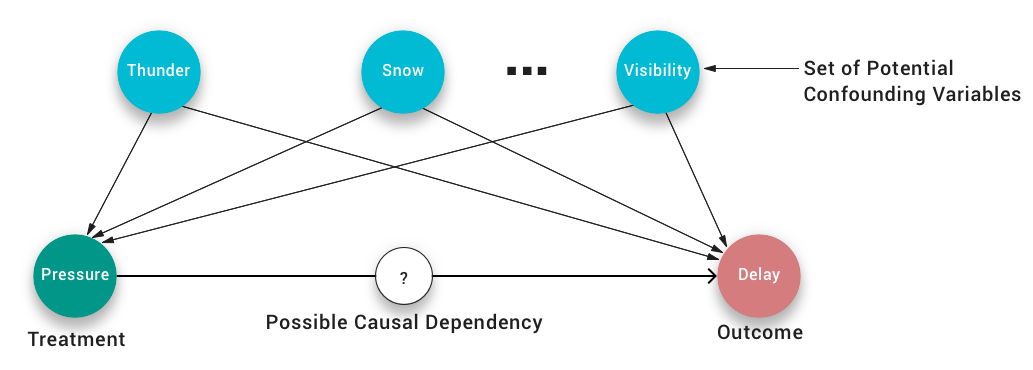
\includegraphics[scale=0.16]{figures/Scenario-Graph.png}
\caption{Confounding influence}
\label{fig:cv}
\vspace{-0.5cm}
\end{figure}
}

% adjusting for confounding variables before
\ignore{{\bf Adjusting for confounding variables:}
In order to draw valid causal conclusions, we need to adjust for confounding influences.
Conceptually, adjusting for one confounding variable is easy.  First, we partition the data into groups with similar confounding influence measures.
 Then, we compute the ATE as the weighted average of the effects \emph{in each group}.
 However, real-world causal inference requires many confounding variables.
  For example, LowPressure has more than ten confounding variables
 (some of them are shown in Fig. \ref{fig:cv}).
 In such a case, the groups often become too specific, lacking enough units in each group to enable a meaningful estimation of the ATE.


 Sophisticated techniques are required to adjust for a large set of confounding variables. \GSQL
 implements two dominant approaches used in social science and statistics, namely,
  {\em coarsened exact matching (CEM)} and {\it propensity score matching (PSM)}
 \cite{IacKinPor09,Rubin1983b}.
 The goal of matching is to prune data so that
the remaining {\em matched} data have better \emph{balance}
between the treated and control groups. That is, the empirical
distributions of the confounding variables in the treated and control
groups are similar after matching.
Once the two groups are balanced, any observed difference of the
outcome between the two groups can be attributed to the treatment. In
our demo, (1)\ for each treatment, we select a set of covariates
deemed to confound the treatment and DepDelay (Figure \ref{sfig:demo-tutorial}c) and
  (2)\ we select a matching method and adjust its tuning parameters.}
% adjusting for confounding variables after 
%\newpage
{\bf Adjusting for confounding variables:}
For the sake of drawing valid conclusions to the causal questions, we must adjust for these confounding variables. Conceptually, adjusting for one confounding variable is easy. It involves partitioning the data into similar groups with similar confounding influence measures. Next, the ATE is computed using the weighted average of the effects \emph{in each group}. However, real world causal inference is much more complicated as it involves many confounding variables. Fig. \ref{fig:cv} shows some of the many confounding variables in this example. In this case, the groups become overly specific and begin to lack enough units to create a meaningful calculation of the ATE.

Sophisticated techniques are required to adjust for a large set of confounding variables. ZaliQL implements two primary approaches that are commonly found in statistics: {\em coarsened exact matching (CEM)} and {\em propensity score matching (PSM)} \cite{IacKinPor09,Rubin1983b}. The goal of matching is to prune data so that the remaining {\em matched} data have greater {\em balance} between the treated and control groups. In other words, the empirical distributions of the confounding variables in the treated and control groups are similar after matching. Once the groups have more or less achieved a sense of balance, the observed difference of the outcome between the two groups can be attributed to the treatment. In our demonstration, we will select a set of covariates deemed to confound the treatments and outcome (Fig. \ref{sfig:demo-tutorial}c) and we will select a matching method and adjust its tuning parameters.

% checking balance before
\ignore{{\bf Checking Balance:}  In this step, we check whether the
matching process  successfully improved the covariates' balance. In particular,
 we compare the distribution for each covariate between the
 treated and control group on the matched data
 (this will be done for all treatments). For this task, \GSQL\  provides
 numerical and visual summaries such as mean difference and quantile-quantile plots:
  see Fig. \ref{sfig:demo-tutorial}(d,e).}
% checking balance after
{\bf Checking balance:} This next step requires verifying that the matching process improved the covariates’ balance. Specifically, we will compare the distribution for each covariate between the treated and control group on the matched data for all treatments. ZaliQL provides both numerical and visual summaries for this step of the process including quartile-quartile and mean difference plots. This can be seen in Fig. \ref{sfig:demo-tutorial}d and Fig. \ref{sfig:demo-tutorial}e.

% answers to our causal questions before
{\bf Answers to our causal questions:}
\ignore{In this step,  we answer the causal questions created at the very first step of the demonstration using
\GSQL. For Q1, we show that LowPressure has no significant causal effect on DepDelay.
We show that other treatments \emph{do} have significant causal effect on departure delays (Q2), and further that these causes are different for different airports in the study (Q3, Figure \ref{sfig:demo-tutorial}(f)).
For Q3, we report the major causes of flight delay at the airports under the study are actually different. We validate the statistical significance of our findings with t-tests, and show that the identified causes match
FAA reports.}
% answers to our causal questions after
Finally, we are able to answer the causal questions created in the first step of our process. For Q1, we will show that LowPressure has no significant causal effect on DepDelay. For Q2, we will identify that other treatments have significant causal effects on DepDelay (Fig. \ref{sfig:demo-tutorial}f). Regarding Q3, we will report that the major causes of flight delay at the airports included in the study are actually different. Two sample z-tests will be used to validate the statistical significance of the results. We will show that the obtained results are validated by FAA reports.

% scalability before
\ignore{{\bf Scalability:} Finally, we demonstrate
  scalability by letting users interactively run queries on this large
   dataset--which would take the existing toolkits hours. As seen in Figure \ref{sfig:demo-tutorial}(g),
\GSQL\ can process 100M entries in less than a few minutes, whereas
existing systems like R, SPSS or SAS,
 take up to an hour to process just 5M entries. \footnote{We note that
   the
   developers of statistical software packages for CEM have identified
   \GSQL\ as a more scalable approach: see \url{http://gking.harvard.edu/cem}.}}
% scalability after
{\bf Scalability:} The last part of this demonstration will allow us to show the scalability by letting users interactively run queries of this large dataset. This process would take existing toolkits hours to complete; however, as seen in Fig. \ref{sfig:demo-tutorial}g, ZaliQL can process 100M entries in less than a few minutes, whereas other systems such as R, SPSS, or SAS, take up to an hour just to process 5M entries.\footnote{We note that the developers of statistical software packages for CEM have identified ZaliQL as a more scalable approach: see \url{http://gking.harvard.edu/cem}.}


\section{Internals}
\subsection{Basic Formalism}

The basic causal model in statistics is called the
\ignore{Neyman-Rubin Causal Model (NRCM) (also referred to as}
{\em potential outcome framework} (POF) \cite{Rubin2005}.
In this model, we are given a table with $N$ rows called {\em units} indexed by $i=1 \ldots N$ (see
Table~ \ref{fig:causal:inference}).  The binary attribute $T$ denotes {\em treatment assignment}.
%sr: already in first para. ($T=1$ means the unit was treated; $T=0$ means the unit was subjected to control);
$X$ is a vector of
background characteristics, (e.g., airport, airline, weather \ldots) of each unit,
called {\em covariates}, unaffected by treatment; and the two
attributes $Y(0), Y(1)$ represent {\em potential outcomes}: $Y(1)$ is
the outcome of the unit if it is exposed to the treatment and $Y(0)$
is the outcome when it is exposed to the control.

%For any attribute $T$, we write $T_i$ for the value of the $i$'s unit.
The {\em treatment effect}
caused by the treatment $T_i$ for the $i$th unit  is defined as $Y_i(1)-Y_i(0)$.
The goal of causal analysis is to compute the {\em average treatment
  effect (ATE)}:   $$ATE = \E[Y(1)-Y(0)] = \E[Y(1)] - \E[Y(0)].$$


\begin{figure}
  \centering
{
  \scalebox{0.7}{\begin{tabular}{|c|c|c|c|c|c|} \hline
    Unit & Covariates & Treatment & Treatment & Control & Causal  Effect \\
   & $X$ & assignment $T$ & outcome $Y(1)$ & outcome $Y(0)$ & $Y(1)-Y(0)$ \\
    \hline
    1 & $X_1$ & $T_1$ & $Y_1(1)$ & $Y_1(0)$ & $Y_1(1) - Y_1(0)$ \\
    2 & $X_2$ & $T_2$ & $Y_2(1)$ & $Y_2(0)$ & $Y_2(1) - Y_2(0)$ \\
    $\ldots$ & $\ldots$ & $\ldots$ & $\ldots$ & $\ldots$ & $\ldots$ \\
    N & $X_N$ & $T_N$ & $Y_N(1)$ & $Y_N(0)$ & $Y_N(1) - Y_N(0)$ \\ \hline
  \end{tabular}}
}
\caption{The Potential Outcome Framework}
  \label{fig:causal:inference}
  \vspace{-3mm}
\end{figure}
\noindent
The so-called {\em fundamental problem of causal inference} %(FPCI)
is that
for each unit we only know either $Y(1)$ or $Y(0)$ but not both.
\ignore{\danp{Can we add an example to make this more intuitive,
 since it's important e.g.: each individual flight has either
    LowPressure=1 or =0, not both}} For example, each individual
flight has either LowPressure=1 or LowPressure=0, so only one of DepDelay(1)
or DepDelay(0) is available for each row.
Thus, further assumptions are needed for estimating ATE. \ignore{
\cite{Holland1986}, and causal inference is reduced to a missing data
problem \cite{RosenbaumRubin1983}. }


The strongest is the {\em independence assumption}:
the treatment mechanism is independent of the potential outcomes,
i.e., $(Y(1), Y(0)) \bigCI T$. This might hold in a properly constructed randomized trial. Then,
$\E[Y(1)]=\E[Y(1)|T=1]$ and similarly $\E[Y(0)]=\E[Y(0)|T=0]$ and so:  $$ATE = \E[Y(1)|T=1]-\E[Y(0)|T=0].$$

However, \GSQL\  is designed for drawing causal inference from {\em
  observational data}, where independence fails in general. \ignore{
For
example, thunder occurs mostly in the summer, which is also high
travel season, and therefore delays may be caused by the high traffic.
In that case $T$ and $Y(0)$ (the delay when thunder does not occur)
are correlated, since they are high in the summer and low in the
winter, and similarly for $T$ and $Y(1)$.  \ignore{The vast majority of datasets
available to analysts today are observational data, and this motivates
our interest in this case.}}  Here, statistical literature makes two standard, weaker
assumptions called {\em Strong
  Ignorability}: for all $x$: \\% the following hold:
  (1)  ${Y(0), Y(1) \bigCI T} | X=x$ (unconfoundedness) and \\
  (2) $0 < \textrm{Pr}(T = 1 | X=x) < 1$ (overlap)~\cite{Rubin1983b}.


If strong ignorability holds, one can estimate ATE by
 taking the  average difference for each group with a particular value of $X$ \ignore{\danp{Need to define
   what a group is here}} i.e., $\E_x[\E[Y(1)-Y(0)| X=x]]$.
In practice, however, a direct application of this method is
impossible, because the data is typically very sparse: for any value
$X=x$ we either have no data values at all, or very few such values,
which means that estimating $\E[Y(T)|T=1\mbox{ or }0,X=x]$ as an
average from the database leads to large sampling error. A solution adopted in
statistics is {\em matching}~\cite{Rubin1983b}.


\subsection{Matching Methods}
\label{sec:algo}
% matching methods before
\ignore{The idea is to match each treated unit to one or multiple control
units with ``close'' values of the covariate attributes $X$
(closeness is defined using some distance function between the covariate values of two units). Given a table $R(T,X_1 \ldots,X_n,Y)$,
 \GSQL\ offers the following two matching methods:}
% matching methods after
This process involves theoretically matching each treated unit to one of multiple control units with similar values of the covariate attributes \cite{IacKinPor09}. Closeness is defined using some distance function between the covariate values of two units. Given a table, $R(T,X_1 \ldots,X_n,Y)$, ZaliQL offers the following two matching methods.

\newpage
{\bf Propensity score matching:}
\label{sec:nnm}
% propensity score matching paragraph 1 before
\ignore{The most common method is $k:1$ nearest neighbor
matching based on {\em propensity score matching} (PSM) \cite{Rubin1983b}.  A propensity score is the probability of a unit being assigned to a particular
treatment given a set of  covariates i.e., $P(x)=P(T=1|X=x)$.  This method
 selects the $k$ best control matches for each individual
in the treatment group, that are closer than a pre-specified {\em caliper}, in a greedy manner.
\GSQL\ estimates propensity score using logistic regression.}
% propensity score matching paragraph 1 after
The most common method is $k:1$ nearest neighbor matching based on {\em propensity score matching (PSM)} \cite{Rubin1983b}. Propensity score is the probability of a unit being assigned to a treatment given a set of covariates (i.e. $P(x)=P(T=1|X=x)$). This method selects the $k$ best control matches for each individual in the treatment group which are closer than a pre-specified {
\em caliper}. ZaliQL estimates propensity score using logistic regression.


% propensity score matching paragraph 2 before 
\ignore{
The basic SQL statement to perform PSM
is depicted in Fig. \ref{fig:nnmnr}.
In this solution,
nearest control units are identified
by means of an anti-join.
Specifically, all potential matches, and their distances, are identified by
joining the treated with the control units that are closer on propensity score than
the caliper. Then, this set is sorted into ascending order of
distances.  In addition, the order of each row in the sorted set is identified
using the window function {\verb|ROW_NUMBER|}.
Finally, $k$ closest controls are selected as the matched units. Note that \GSQL\  generates more efficient SQL statements by
leveraging recent developments in  spatial-databases
(see e.g., \cite{obe2015postgis}).}
% propensity score matching paragraph 2 after
The basic SQL statement to perform PSM is depicted in Fig. \ref{fig:nnmnr}. In this solution, nearest control units are identified by means of an anti-join. In other words, all potential matches, and their distances, are identified by joining the treated with the control units that are closer on propensity score than the caliper. Then, this set is sorted in ascending order of distances. Additionally, the order of each row in the sorted set is identified using the window function {\verb|ROW_NUMBER|}. Finally, $k$ closest controls are selected as the matched units. Note that \GSQL\  generates more efficient SQL statements using recent developments in spatial-databases (see e.g., \cite{obe2015postgis}).


\begin{figure}
  \centering
\begin{alltt} \scriptsize
CREATE VIEW PSM_Matched
AS WITH potential_matches AS
  (SELECT treated.ID AS tID, control.ID AS cID,
          abs(Treated.PS-Control.PS)  AS distance
   FROM \(\rel\) AS control, \(\rel\) AS treated
   WHERE control.T=0 AND treated.T=1
     AND abs(Treated.PS-Control.PS) < \(caliper\))),
            ordered_potential_matches AS
  (SELECT *, ROW_NUMBER() over (ORDER BY distance) AS order
   FROM potential_matches)
SELECT *
FROM ordered_potential_matches AS rp
WHERE NOT EXISTS
    (SELECT *
     FROM ordered_potential_matches AS z
     WHERE z.order < opm.order AND z.cID=opm.cID)
  AND (SELECT count(*)
     FROM ordered_potential_matches AS opm
     WHERE z.order < opm.order AND z.tID=opm.tID)\( \leq k\);
\end{alltt} \vspace{-.3cm}
  \caption{ Propensity score matching}\label{fig:nnmnr}
\end{figure}


\begin{figure}
\begin{alltt} \scriptsize
CREATE VIEW CEM_Matched AS
WITH subclasses AS
  (SELECT *,
          max(ID) OVER w subclass, max(T) AS min_treatment,
          min(T)AS max_treatment
   FROM \(\crele\)
   Group by \(\ccv\)
   Having min_treatment!=max_treatment)
SELECT *
FROM subclasses,\(\crele\)
WHERE subclasses.\(\ccv\)=\(\crele\).\(\ccv\)

\end{alltt}
\vspace{-.45cm}
  \caption{Coarsened Exact Matching}\label{fig:cem}
\end{figure}



{\bf Coarsened exact matching (CEM):}
% cem paragraph 1 before
\ignore{In this method the vector of covariates $\cv$ is
coarsened according to a set of user-defined cutpoints or any
automatic discretization algorithm.
\ignore{CEM has officially been "Qualified for Scientific Use" by the U.S. Food and Drug Administration\cite{IacKinPor09}.}
All units with similar coarsened
covariate values are placed in unique groups. All
groups with at least one treated and one control unit are retained
and the rest of units are discarded.  Let $\ccv$ be the
coarsened version of $\cv$ and $R^c$ be a coarsened
version of R. As depicted in Fig. \ref{fig:cem},
CEM is essentially a GROUP-BY-HAVING query.
\GSQL\  also supports several supervised and unsupervised methods for coarsening% proposed in
~\cite{dougherty1995supervised}.}
% cem paragraph 1 after
In this method, the vector of covariates $\cv$ is coarsened according to a set of user-defined cut points or with a discretization algorithm. All units with similar coarsened covariate values are placed in unique groups. Then, groups with at least one treated and one control unit are retained while all others are discarded from data. We let $\ccv$ be the coarsened version of $\cv$ and $R^c$ be a coarsened version of R. As depicted in Fig. \ref{fig:cem}, CEM is essentially a GROUP-BY-HAVING query. 

% cem paragraph 2 before
\ignore{We observed that CEM is an {\em Iceberg query}.  These are  GROUP-BY-HAVING queries
in which the output size is typically much smaller than the input (the
tip of an iceberg). Iceberg queries have been studied
extensively in databases and data mining (see e.g.,
\cite{fang1999computing,findlater2003iceberg}).
\GSQL\ leverages these techniques to efficiently compute CEM for several treatments simultaneously.}
% cem paragraph 2 after
We observed that CEM is an ``Iceberg query'' in the sense that it is a GROUP-BY-HAVING query where the output size is typically much smaller than the input (i.e. the tip of an iceberg). Iceberg queries have been studied extensively in databases and data mining \cite{fang1999computing,findlater2003iceberg}. ZaliQL leverages these techniques and the prior research on them in order to more efficiently compute CEM for several treatments simultaneously, giving it a strong advantage over other softwares.


{\bf Analysis after matching:} After a balanced and matched subset of data is extracted, ATE can be computed. ZaliQL supports a wide range of statistical tests such as z-test, t-test, egression-based tests , and Chi-square test to compute the statistical significant of the treatment group.


\section{Conclusions}
% conclusion before
\ignore{In this demonstration, we introduce \GSQL: a tool for
performing causal inference
on large relational data within a DBMS. \GSQL\ makes the first step towards truly scalable causal inference by modeling it as a data management problem. \GSQL\ implements a wide range of methods for causal inference developed in statistics with existing techniques
in data management. This provides scalable evaluation of several causal hypotheses
on relational data.}
% conclusion after
In this demonstration, we will introduce ZaliQL, a tool for performing causal inference on large relational data within a DBMS. ZaliQL makes the first step towards truly scalable causal inference by modeling it as a data management problem. ZaliQL implements a wide range of methods for causal inference developed in statistics with existing techniques in data management. This provides scalable evaluation of several causal hypothesis on relational data. Overall, this demonstration will serve as both an introduction to causal inference and an illustration of the vast benefits ZaliQL possesses over traditional statistical analysis packages.


\section{ACKNOWLEDGEMENTS}
This work is supported in part by the National Science Foundation through NSF grants IIS-1614738 and
University of Washington's CSE Postdoc Research Award.

% The following two commands are all you need in the
% initial runs of your .tex file to
% produce the bibliography for the citations in your paper.
\bibliographystyle{abbrv}
\bibliography{vldb_sample}  % vldb_sample.bib is the name of the Bibliography in this case
% You must have a proper ".bib" file
%  and remember to run:
% latex bibtex latex latex
% to resolve all references


\end{document}
